\chapter{Crosstalk}
Nelle interconnessioni e nei sistemi multiconductor, il crosstalk (o diafonia) rappresenta l'accoppiamento elettromagnetico indesiderato tra canali o linee adiacenti. Il rumore di crosstalk riduce le prestazioni del sistema e introduce problematiche aggiuntive, quali l'emissione elettromagnetica e la suscettività a campi esterni.

L'interazione tra conduttori è riconducibile a due sorgenti fisiche fondamentali:
\begin{itemize}
    \item \textbf{Accoppiamento elettrico} $\rightarrow$ mediato dalla capacità mutua $C_m$ tra i conduttori (accoppiamento capacitivo dovuto al campo elettrico).
    \item \textbf{Accoppiamento magnetico} $\rightarrow$ mediato dall'induttanza mutua $L_m$ tra i circuiti (accoppiamento induttivo dovuto al campo magnetico).
    \item \textbf{Accoppiamento combinato} $\rightarrow$ sovrapposizione simultanea degli effetti capacitivo e induttivo.
\end{itemize}
\begin{figure}[H]
	\centering
	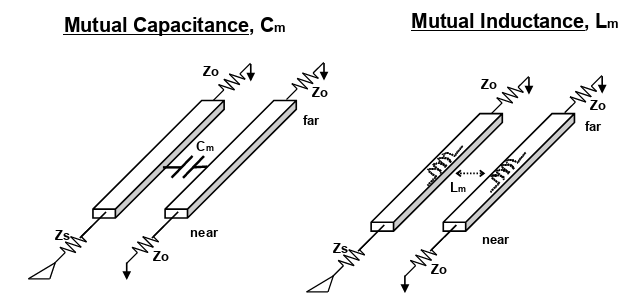
\includegraphics[width=0.7\linewidth]{immagini/crosstalk1}
\end{figure}

La configurazione classica comprende un circuito aggressore (canale attivo), alimentato da una sorgente $V_s$ con resistenza interna $R_s$ e terminato sul carico $R_L$, e un circuito vittima (canale passivo), terminato su due resistenze d'estremità: la resistenza di near-end $R_{\text{NE}}$ e la resistenza di far-end $R_{\text{FE}}$.
\begin{figure}[H]
	\centering
	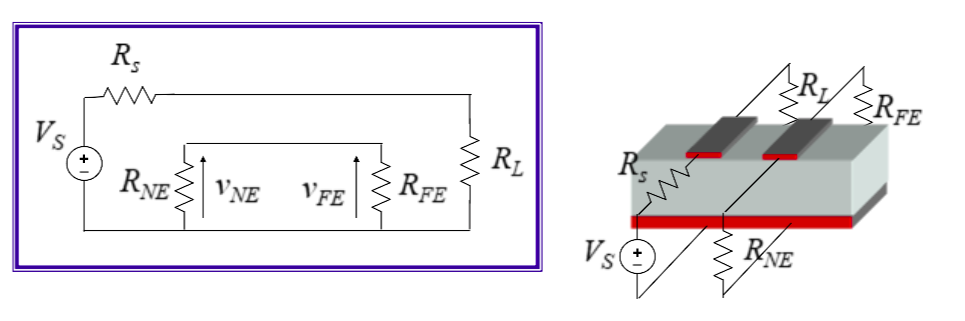
\includegraphics[width=0.65\linewidth]{immagini/crosstalk2}
\end{figure}
La tensione e la corrente presenti sul canale attivo generano rispettivamente campo elettrico e campo magnetico variabili nel tempo, inducendo tensioni e correnti sul canale passivo. Si definiscono le due grandezze di rumore terminali:
\begin{itemize}
    \item \textbf{NEXT (Near-End Crosstalk)} $\rightarrow$ rumore di crosstalk rilevato all'estremità vicina alla sorgente ($V_{\text{NE}}$).
    \item \textbf{FEXT (Far-End Crosstalk)} $\rightarrow$ rumore di crosstalk rilevato all'estremità lontana dal generatore ($V_{\text{FE}}$).
\end{itemize}

\section{Definizione dei parametri parassiti di accoppiamento}
Nei sistemi multiconductor (come piste microstrip su piano di massa o conduttori affiancati), i parametri distribuiti trasversi descrivono la matrice di capacità e di induttanza per unità di lunghezza.

Per una coppia di conduttori in presenza di massa:
\begin{itemize}
    \item \textbf{Capacità mutua ($C_m$)} $\rightarrow$ lega la carica indotta sulla linea passiva alla tensione della linea attiva. Le relazioni costitutive cariche-tensioni sono espresse dal sistema:
    \begin{figure}[H]
    	\centering
    	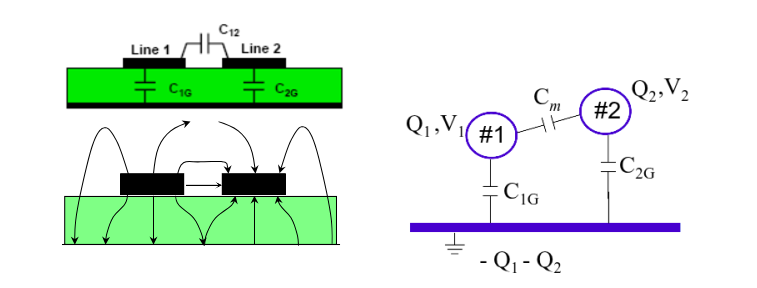
\includegraphics[width=0.6\linewidth]{immagini/crosstalk3}
    \end{figure}
    \[
    \begin{cases}
    Q_1 = (C_{1G} + C_m) V_1 - C_m V_2 \\
    Q_2 = -C_m V_1 + (C_{2G} + C_m) V_2
    \end{cases}
    \]
    La matrice delle capacità assume la forma:
    \[
    \mathbf{C} = \begin{bmatrix} C_{1G} + C_m & -C_m \\ -C_m & C_{2G} + C_m \end{bmatrix}
    \]
    \item \textbf{Induttanza mutua ($L_m$)} $\rightarrow$ quantifica il flusso magnetico concatenato con il circuito passivo dovuto alla corrente circolante nel canale attivo. I flussi concatenati con i due conduttori si esprimono mediante la matrice delle induttanze:
    \begin{figure}[H]
    	\centering
    	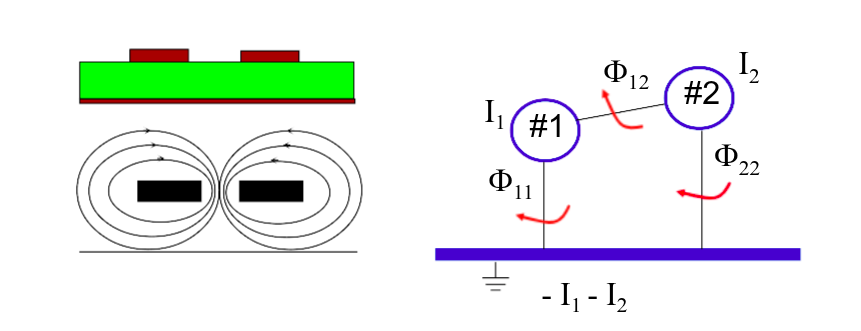
\includegraphics[width=0.6\linewidth]{immagini/crosstalk4}
    \end{figure}
    \[
    \begin{cases}
    	\Phi_1 = L_{11} I_1 + L_m I_2 \\
    	\Phi_2 = L_m I_1 + L_{22} I_2
    \end{cases}
    \]
    \[
    \mathbf{L} = \begin{bmatrix} L_{11} & L_{12} \\ L_{21} & L_{22} \end{bmatrix} = \begin{bmatrix} L_{11} & L_m \\ L_m & L_{22} \end{bmatrix}
    \]
\end{itemize}




\section{Modello per linee elettricamente corte}
Quando la lunghezza geometrica delle linee $l$ è molto minore della lunghezza d'onda del segnale:
\[
l \ll \lambda
\]
e sussiste la condizione di \textbf{accoppiamento debole}:
\[
\frac{L_m}{\sqrt{L_1 L_2}} \ll 1, \qquad \frac{C_m}{\sqrt{C_1 C_2}} \ll 1
\]
l'analisi della diafonia si semplifica tramite la \textbf{sovrapposizione} degli effetti induttivo e capacitivo calcolati a parametri concentrati. In tali condizioni, la presenza della linea vittima non perturba significativamente le grandezze sul canale aggressore.
\begin{figure}[H]
	\centering
	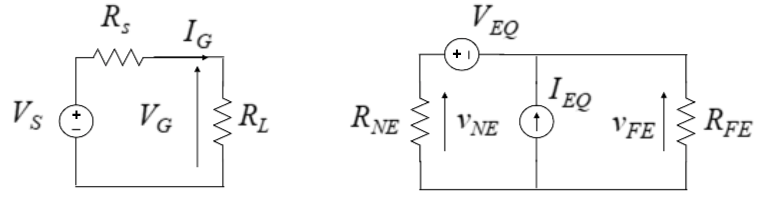
\includegraphics[width=0.6\linewidth]{immagini/crosstalk5}
\end{figure}

La corrente e la tensione non perturbate sul canale aggressore si valutano in regime stazionario o a bassa frequenza:
\[
I_G^{\text{DC}} = \frac{V_s}{R_s + R_L}, \qquad V_G^{\text{DC}} = \frac{R_L V_s}{R_s + R_L}
\]
I generatori equivalenti sulla linea vittima risultano proporzionali alla derivata temporale (o alla pulsazione $\omega$ nel dominio dei fasori) delle grandezze dell'aggressore:
\[
V_{\text{EQ}} = j\omega L_m I_G^{\text{DC}}, \qquad I_{\text{EQ}} = j\omega C_m V_G^{\text{DC}}
\]

La tensione di near-end e di far-end sul circuito vittima è pari alla somma algebrica dei contributi induttivi e capacitivi:
\[
\frac{V_{\text{NE}}}{V_s} = j\omega (M_{\text{IND}} + M_{\text{CAP}})
\]
\[
\frac{V_{\text{FE}}}{V_s} = j\omega (-M_{\text{IND}} + M_{\text{CAP}})
\]
Gli indici di accoppiamento induttivo $M_{\text{IND}}$ e capacitivo $M_{\text{CAP}}$ sono determinati dalle impedenze terminali e dai parametri mutui:
\[
M_{\text{IND}} = \frac{R_{\text{NE}}}{R_{\text{NE}} + R_{\text{FE}}} \frac{L_m}{R_s + R_L}
\]
\[
M_{\text{CAP}} = \frac{R_{\text{NE}} R_{\text{FE}}}{R_{\text{NE}} + R_{\text{FE}}} \frac{R_L C_m}{R_s + R_L}
\]

\subsection{Differenza tra NEXT e FEXT}
La dissimmetria fondamentale tra crosstalk di near-end e quella di far-end risiede nella direzione delle correnti indotte:
\begin{itemize}
    \item La corrente generata dall'induttanza mutua $I_{Lm}$ circola nel circuito vittima in verso opposto alla corrente dell'aggressore, fluendo dal far-end verso il near-end.
    \item La corrente iniettata dalla capacità mutua $I_{Cm}$ si suddivide equamente ai due capi se le terminazioni sono identiche, dirigendosi verso massa sia a near-end che a far-end.
\end{itemize}
\begin{figure}[H]
	\centering
	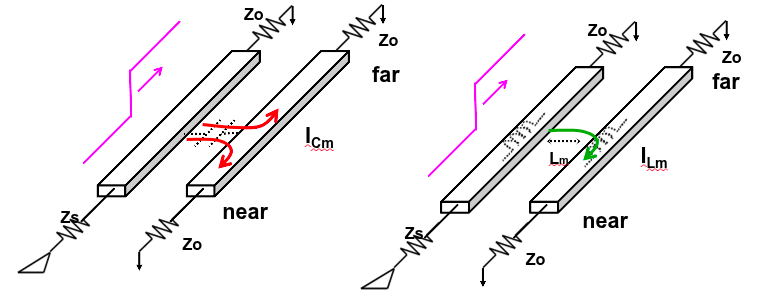
\includegraphics[width=0.6\linewidth]{immagini/crosstalk6}
\end{figure}
Le correnti risultanti soddisfano le relazioni:
\[
I_{\text{near}} = I_{Cm} + I_{Lm}
\]
\[
I_{\text{far}} = I_{Cm} - I_{Lm}
\]
Ne consegue che a near-end gli effetti capacitivo e induttivo si sommano costruttivamente, mentre a far-end si sottraggono.

\subsection{Comportamento in frequenza al variare delle impedenze di carico}
La natura dominante dell'accoppiamento dipende dal rapporto tra l'impedenza del circuito aggressore e quella del carico:
\begin{itemize}
    \item \textbf{Condizione a bassa impedenza ($R_L \ll R_s$)} $\rightarrow$ nel canale attivo scorrono correnti elevate mentre le tensioni rimangono contenute; l'accoppiamento è prevalentemente induttivo ($M_{\text{IND}} \gg M_{\text{CAP}}$).
    \begin{figure}[H]
    	\centering
    	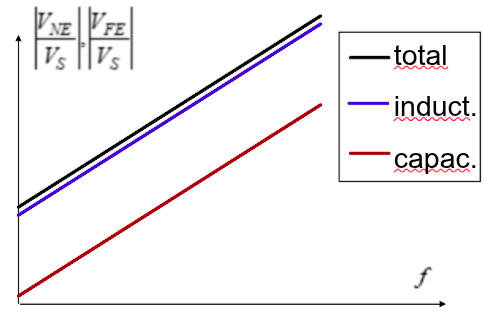
\includegraphics[width=0.4\linewidth]{immagini/crosstalk7}
    \end{figure}
    \item \textbf{Condizione ad alta impedenza ($R_L \gg R_s$)} $\rightarrow$ nel canale attivo si manifestano tensioni elevate con deboli correnti; l'accoppiamento è prevalentemente capacitivo ($M_{\text{CAP}} \gg M_{\text{IND}}$).
    \begin{figure}[H]
    	\centering
    	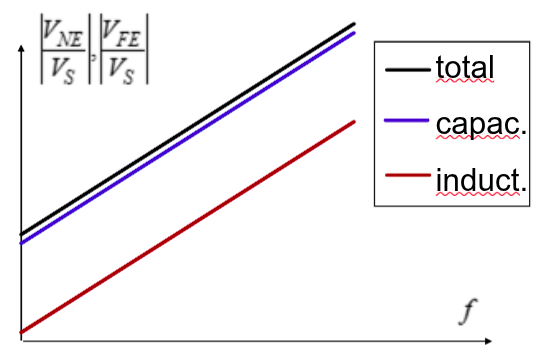
\includegraphics[width=0.4\linewidth]{immagini/crosstalk8}
    \end{figure}
\end{itemize}

In entrambe le condizioni, nella regione a parametri concentrati la tensione indotta cresce linearmente con la frequenza con una pendenza di $+20\text{ dB/decade}$.

\section{Modello per linee elettricamente lunghe}
All'aumentare della frequenza o della lunghezza fisica del collegamento, la condizione di linea elettricamente corta decade:
\[
l \approx \lambda \quad \text{oppure} \quad l > \lambda
\]
In questo regime le interconnessioni devono essere trattate mediante la teoria delle linee di trasmissione multiconductor (MTL - Multiconductor Transmission Lines).

\subsection{Formulazione matriciale MTL}
Il comportamento elettromagnetico lungo la coordinata longitudinale di propagazione è descritto dalle equazioni dei telegrafisti in forma vettoriale-matriciale:
\begin{itemize}
    \item \textbf{Nel dominio del tempo (linee ideali senza perdite):}
    \[
    -\frac{\partial \mathbf{v}(x,t)}{\partial x} = \mathbf{L} \frac{\partial \mathbf{i}(x,t)}{\partial t}
    \]
    \[
    -\frac{\partial \mathbf{i}(x,t)}{\partial x} = \mathbf{C} \frac{\partial \mathbf{v}(x,t)}{\partial t}
    \]
    \item \textbf{Nel dominio della frequenza (linee reali con perdite):}
    \[
    -\frac{d \mathbf{V}(z,\omega)}{dz} = \mathbf{Z}(z,\omega) \mathbf{I}(z,\omega)
    \]
    \[
    -\frac{d \mathbf{I}(z,\omega)}{dz} = \mathbf{Y}(z,\omega) \mathbf{V}(z,\omega)
    \]
    dove $\mathbf{Z} = \mathbf{R} + j\omega\mathbf{L}$ e $\mathbf{Y} = \mathbf{G} + j\omega\mathbf{C}$.
\end{itemize}
\begin{figure}[H]
	\centering
	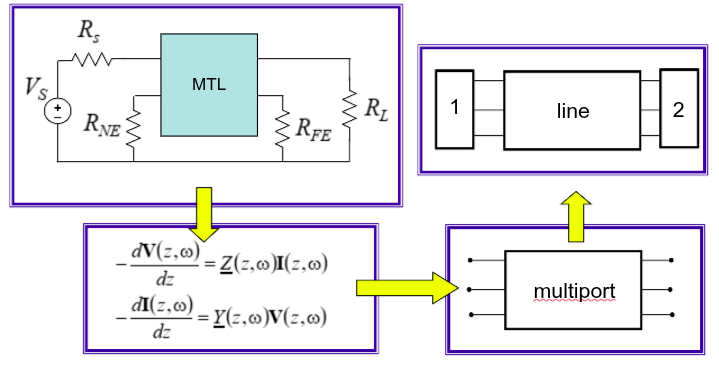
\includegraphics[width=0.7\linewidth]{immagini/crosstalk9}
\end{figure}

\subsection{Risposta nel dominio del tempo e confronto tra modelli}
I fasci di cavi (cable bundles) presentano un'elevata sensibilità al crosstalk e all'accoppiamento con campi elettromagnetici esterni. Considerando una coppia di conduttori paralleli in prossimità di un piano metallico di massa con parametri distribuiti tipici:
\begin{itemize}
    \item $L_{11} = L_{22} = 309\text{ nH/m}$, $L_m = 21.7\text{ nH/m}$
    \item $C_{11} = C_{22} = 144\text{ pF/m}$, $C_m = -6.4\text{ pF/m}$
    \item $\mathbf{R} = \text{diag}(0.524\ \Omega/\text{m})$, $\mathbf{G} = \text{diag}(0.905\text{ mS/m})$
    \item Impedenza caratteristica $Z_0 \approx 50\ \Omega$
\end{itemize}
\begin{figure}[H]
	\centering
	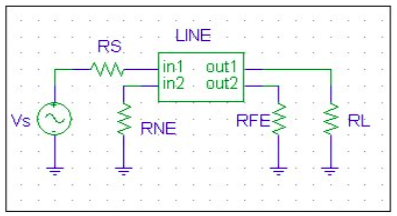
\includegraphics[width=0.4\linewidth]{immagini/crosstalk10}
\end{figure}
si riscontrano i seguenti comportamenti:
\begin{itemize}
    \item \textbf{Ampiezza del disturbo impulsivo} $\rightarrow$ per un gradino con tempo di salita (rise-time) di $1\text{ ns}$ su una linea adattata di lunghezza $10\text{ m}$, il picco di crosstalk raggiunge livelli comparabili alla soglia logica di commutazione ($V_{\text{th}}$), potendo causare false transizioni nei circuiti digitali.
    \begin{figure}[H]
    	\centering
    	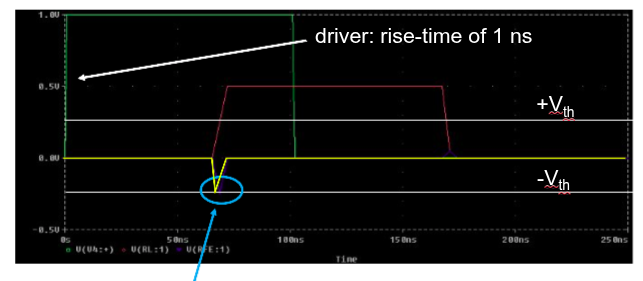
\includegraphics[width=0.6\linewidth]{immagini/crosstalk11}
    \end{figure}
    \item \textbf{Influenza delle perdite} $\rightarrow$ l'inclusione delle perdite ohmiche e dielettriche del cavo non riduce in modo significativo il picco di diafonia rispetto al caso lossless.
    \begin{figure}[H]
    	\centering
    	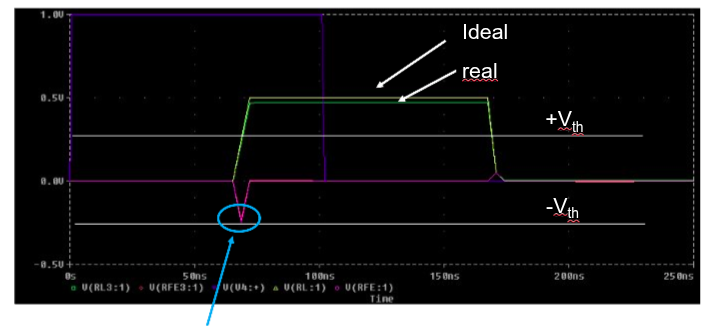
\includegraphics[width=0.6\linewidth]{immagini/crosstalk12}
    \end{figure}
    \item \textbf{Limite di validità del modello a costanti concentrate} $\rightarrow$ il modello a parametri concentrati è accurato solo a basse frequenze (ottimo accordo fino a circa $1\text{ MHz}$ per $l = 10\text{ m}$, e fino a $3\text{ MHz}$ per $l = 3\text{ m}$). A frequenze superiori emergono effetti di risonanza e propagazione d'onda che richiedono il modello distribuito.
    \begin{figure}[H]
    	\centering
    	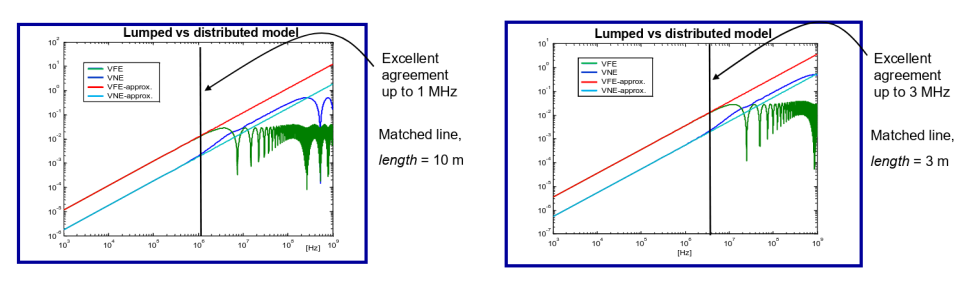
\includegraphics[width=1\linewidth]{immagini/crosstalk13}
    \end{figure}
    \item \textbf{Effetto del disadattamento di impedenza} $\rightarrow$ terminazioni non adattate (es. $R_{\text{NE}} = R_{\text{FE}} = R_L = 0.1 Z_0$) esaltano fortemente le oscillazioni e l'ampiezza della tensione di far-end $V_{\text{FE}}$ rispetto alla condizione perfettamente adattata.
    \begin{figure}[H]
    	\centering
    	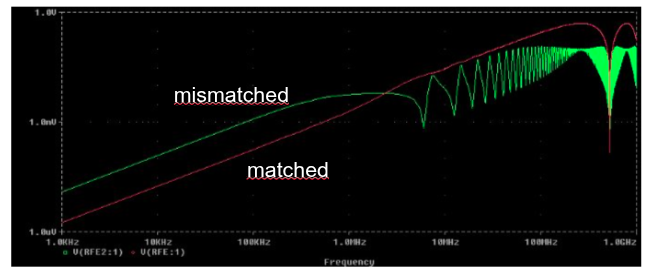
\includegraphics[width=0.6\linewidth]{immagini/crosstalk14}
    \end{figure}
\end{itemize}


\section{Tecniche di riduzione del rumore di crosstalk}
La riduzione dell'interazione parassita tra i canali si consegue mediante l'adozione di schermature, configurazioni twisted-pair e regole mirate di layout su circuito stampato.

\subsection{Schermatura del circuito vittima}
L'impiego di uno schermo metallico cilindrico attorno al conduttore vittima mitiga i due meccanismi di accoppiamento secondo principi distinti:
\begin{itemize}
    \item \textbf{Riduzione dell'accoppiamento capacitivo} $\rightarrow$ 
    Uno schermo interposto ma non connesso a massa non offre alcun beneficio. Se lo schermo non è collegato a terra, la capacità mutua effettiva tra aggressore e circuito interno rimane sostanzialmente invariata:
    \begin{figure}[H]
    	\centering
    	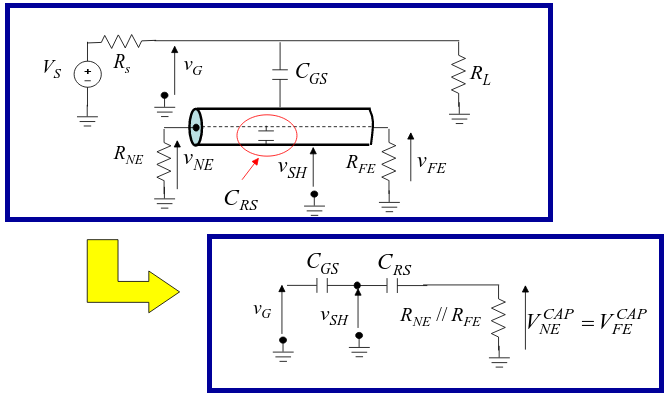
\includegraphics[width=0.6\linewidth]{immagini/crosstalk15}
    \end{figure}
    \[
    C_m = \frac{C_{\text{RS}} C_{\text{GS}}}{C_{\text{RS}} + C_{\text{GS}}} \approx C_{\text{GS}} \qquad (\text{per } C_{\text{RS}} \gg C_{\text{GS}})
    \]
    dove $C_{\text{RS}}$ è la capacità tra aggressore e schermo e $C_{\text{GS}}$ è la capacità tra schermo e conduttore interno.
    Di conseguenza, il coefficiente di accoppiamento capacitivo non viene alterato:
    \[
    M_{\text{SH}}^{\text{CAP}} \approx M_{\text{CAP}}
    \]
    Lo schermo è efficace contro il campo elettrico \textbf{esclusivamente se collegato a massa}: in tal caso il potenziale dello schermo viene vincolato a zero ($V_{\text{SH}} = 0$) e il fattore di accoppiamento capacitivo si annulla:
    \[
    M_{\text{SH}}^{\text{CAP}} = 0
    \]
    \begin{figure}[H]
    	\centering
    	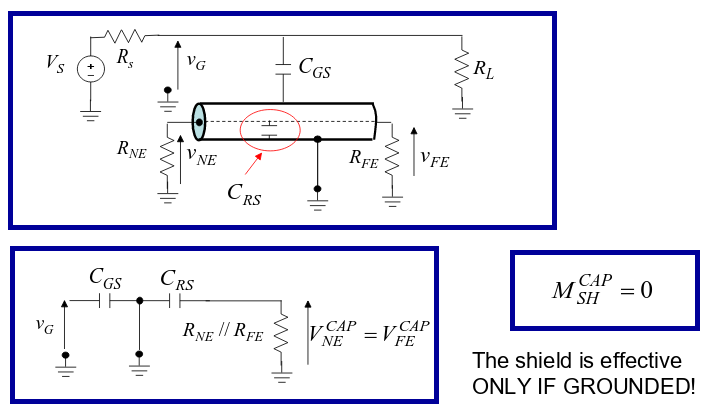
\includegraphics[width=0.6\linewidth]{immagini/crosstalk16}
    \end{figure}
    
    \item \textbf{Riduzione dell'accoppiamento induttivo} $\rightarrow$ 
    Se \textbf{entrambi i capi dello schermo sono collegati a massa}, nel circuito chiuso dello schermo può scorrere una corrente indotta dal campo magnetico esterno. Tale corrente genera un flusso magnetico di reazione che si oppone al flusso incidente, abbattendo la tensione indotta induttivamente:
    \begin{figure}[H]
    	\centering
    	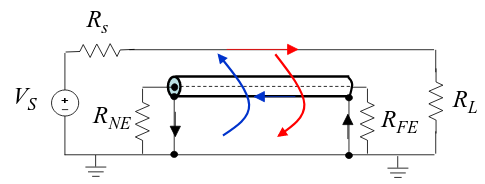
\includegraphics[width=0.5\linewidth]{immagini/crosstalk17}
    \end{figure}
    \[
    V_{\text{NE}}^{\text{IND}} = -V_{\text{FE}}^{\text{IND}} = M_{\text{IND}} \frac{R_{\text{SH}}}{R_{\text{SH}} + j\omega L_{\text{SH}}} V_s
    \]
    dove $R_{\text{SH}}$ e $L_{\text{SH}}$ rappresentano la resistenza e l'induttanza serie dello schermo.
    
    Sotto la frequenza di taglio determinata da:
    \[
    f_c = \frac{R_{\text{SH}}}{2\pi L_{\text{SH}}}
    \]
    la tensione indotta cresce con pendenza $+20\text{ dB/decade}$. Al di sopra di $f_c$, l'effetto di reazione dello schermo limita il disturbo a un valore costante ($0\text{ dB/decade}$).
    \begin{figure}[H]
    	\centering
    	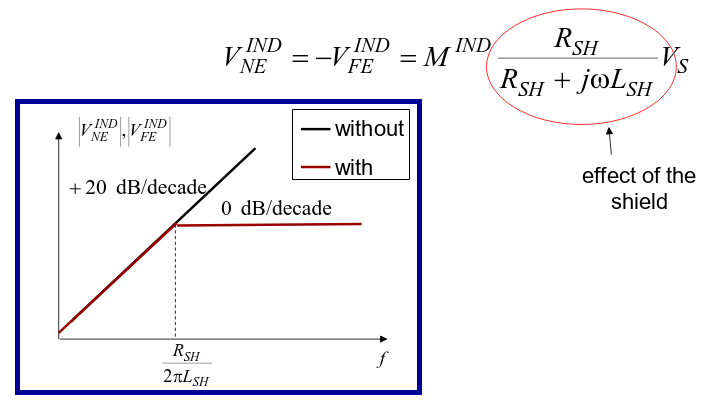
\includegraphics[width=0.6\linewidth]{immagini/crosstalk18}
    \end{figure}
    
    \item \textbf{Regola di messa a terra per conduttori lunghi} $\rightarrow$ per schermi o conduttori elettricamente estesi non è sufficiente collegare a massa una o due estremità; lo schermo deve essere connesso a terra a intervalli regolari pari ad almeno:
    \[
    \Delta l \le \frac{\lambda}{10}
    \]
    \begin{figure}[H]
    	\centering
    	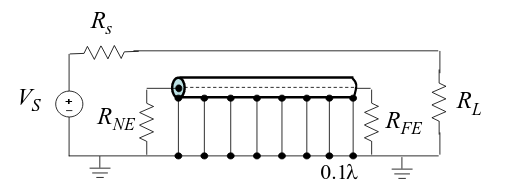
\includegraphics[width=0.5\linewidth]{immagini/crosstalk19}
    \end{figure}
\end{itemize}

\subsection{Cavi a coppia intrecciata (twisted pair)}
L'intreccio dei conduttori del circuito vittima costituisce un metodo efficace per ridurre la diafonia:
\begin{itemize}
    \item L'accoppiamento induttivo viene sistematicamente ridotto in qualsiasi condizione di carico.
    \item L'accoppiamento capacitivo viene ridotto \textbf{esclusivamente in presenza di carichi bilanciati}.
\end{itemize}
Tale principio trova impiego standard nei cavi UTP, FTP e STP (ad esempio in cablaggi ADSL ed Ethernet).
\begin{figure}[H]
	\centering
	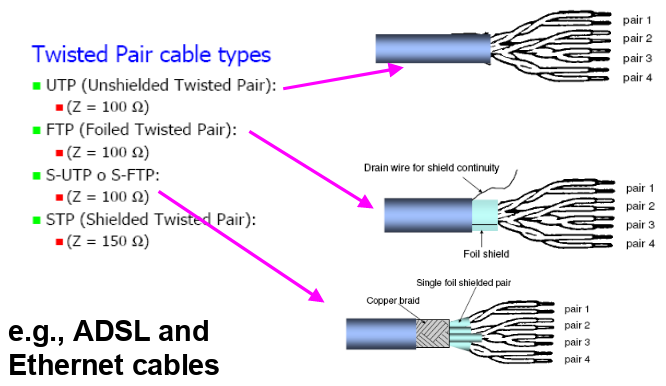
\includegraphics[width=0.6\linewidth]{immagini/crosstalk20}
\end{figure}

Un cavo ritorto è modellabile come una cascata di anelli adiacenti di lunghezza di passo $L_s$:
\begin{itemize}
    \item \textbf{Cancellazione induttiva} $\rightarrow$ due anelli adiacenti intercettano il campo magnetico con orientazione opposta, generando forze elettromotrici indotte $E_1$ ed $E_2$ con polarità alternate che si elidono a vicenda. In una linea con un numero pari di spire l'accoppiamento induttivo si cancella completamente; con un numero dispari di spire residua il contributo di un solo anello elementare.
    \begin{figure}[H]
    	\centering
    	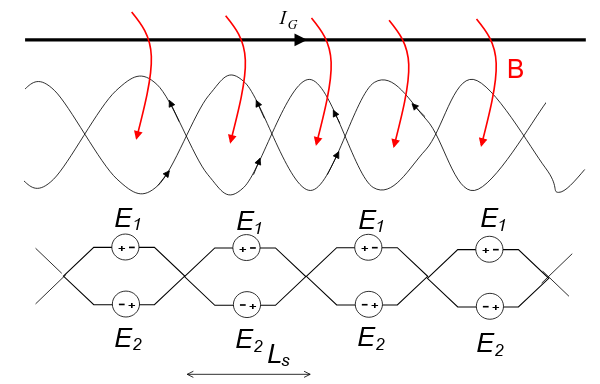
\includegraphics[width=0.5\linewidth]{immagini/crosstalk21}
    \end{figure}
    \item \textbf{Cancellazione capacitiva e bilanciamento dei carichi} $\rightarrow$ le correnti capacitive $I_1$ e $I_2$ iniettate nei conduttori adiacenti si compensano solo se attraversano carichi simmetrici ($R_{\text{NE}}$, $R_{\text{FE}}$). Con carichi bilanciati, le correnti generate da due anelli consecutivi fluiscono sulle resistenze terminali in direzioni opposte, determinando la reciproca cancellazione della tensione ai capi dei carichi. Se i carichi non sono bilanciati, le correnti non si compensano e il disturbo capacitivo persiste.
    \begin{figure}[H]
    	\centering
    	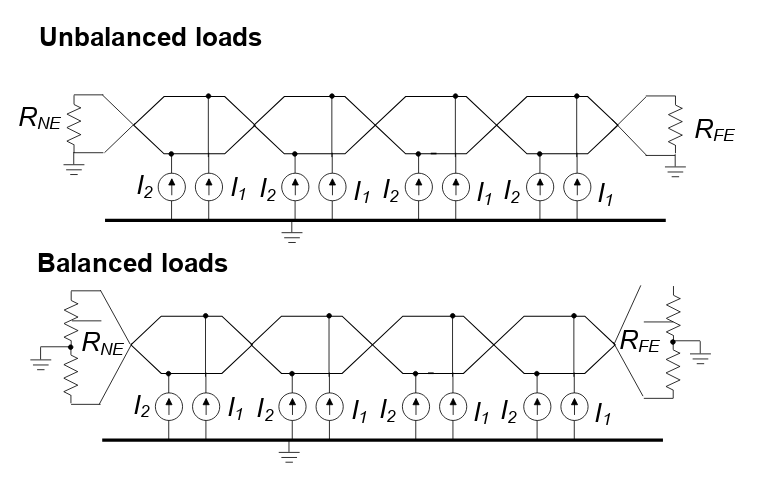
\includegraphics[width=0.6\linewidth]{immagini/crosstalk23}
    \end{figure}
\end{itemize}

\subsection{Accorgimenti di layout e instradamento su PCB}
Nei circuiti stampati, qualora non sia possibile aumentare la distanza fisica di separazione tra le piste, si adottano le seguenti soluzioni:
\begin{itemize}
    \item \textbf{Piste di guardia (guard traces)} $\rightarrow$ inserimento di una pista metallica collegata a massa tra la linea aggressore attiva e la linea passiva (es. tra segnali di clock e linee di segnale sensibili), realizzando una schermatura planare integrata.
    \begin{figure}[H]
    	\centering
    	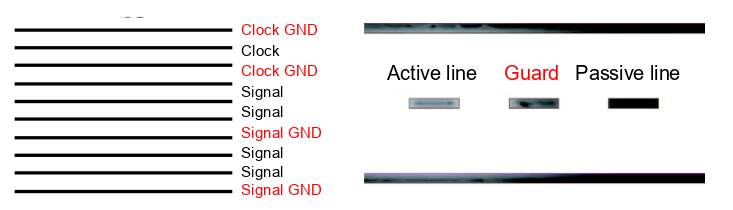
\includegraphics[width=0.6\linewidth]{immagini/crosstalk24}
    \end{figure}
    \item \textbf{Tracciati a serpentina (serpentine routing)} $\rightarrow$ utilizzati convenzionalmente per equalizzare i ritardi di propagazione tra piste parallele (lunghezze $L_p$ e spaziatura $S$), agiscono come un equivalente planare della ritorsione (twisting), abbattendo l'accoppiamento induttivo complessivo.
    \begin{figure}[H]
    	\centering
    	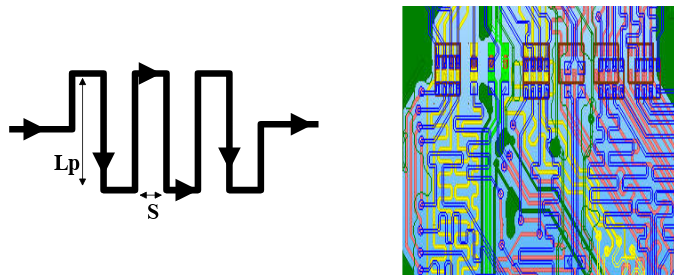
\includegraphics[width=0.6\linewidth]{immagini/crosstalk25}
    \end{figure}
\end{itemize}
